\chapter{Machine learning approach}
\label{ch:MachineLearning}
\graphicspath{{Chapter4/Chapter4Figures/}}
The previous chapter briefly described the basic workings of the optical mark recognition(OCR) system inside the automatic test grader. There is still one critical piece of information that has not been observed in the system. This information is the characters that the student writes into the designated boxes.

\nomenclature[dcnnAcronym]{$DCNN$}{Deep convolutional neural network}
This next chapter will provide two machine learning approaches to significantly improve the accuracy of the system over the previous basic model alone. Firstly an approach to locate and classify hand written characters, provided by the students, using a deep convolutional neural network(DCNN), will be described. A more accurate method in determining the true digit represented by the bubble evidence, using a probabilistic  graphical model(PGM), will also be implemented. This method will then allow for an integrated probabilistic approach to determine the true answer using the character and bubble evidence.

For a more detailed explanation on the DCNN used in this thesis please refer to Appendix \ref{sec:DCNN}.

\section{Character recognition using a neural network}

\subsection{Introduction}
\nomenclature[dcnnAcronym]{$ANN$}{Artificial neural network}

An neural network is a powerful machine learning tool for approximating complex functions. The basic architecture of an neural network can be seen in Figure \ref{fig:nn}. The structure of an feed-forward neural network consist of an input, hidden and output layer, as described in \citet{MichealN2015}. A artificial neural network(ANN) is a simplified approximation of how neurons in the brain works. Each neuron in the network acts as a small processing unit. The final output can thus be collected by reading the value at the output layer after it has been passed each layer of the network.

For this thesis a neural network will be trained to predict what digit(0-9) are most likely present in a image.  Figure \ref{fig:mnist} illustrates the input of of the neural network using and 14 by 14 example image. For this thesis a 28 by 28 greyscalled image will be used as input. Thus if each pixel is 1 value(0.0-1.0) there will be a total of 748 input values. 

\begin{figure}
  \centering
  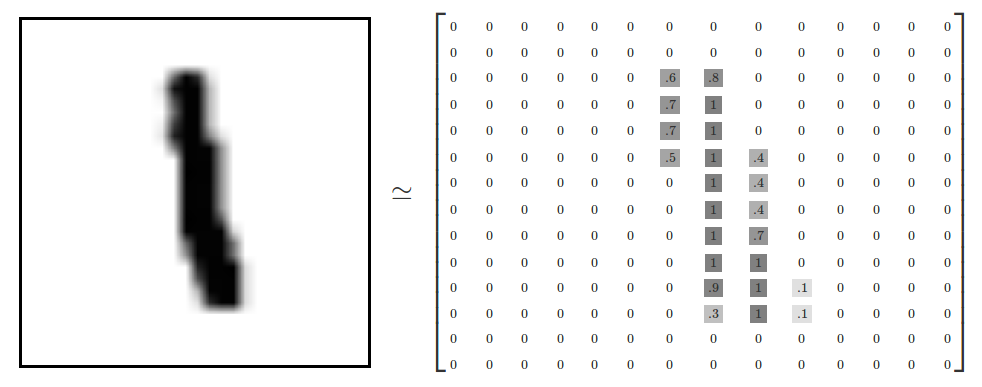
\includegraphics[width=14cm]{MNIST}\\
  \caption{Example image used as input to the neural network, \citet{tensor2017}}%, \citet{tensor2017}
  \label{fig:mnist}
\end{figure}



\subsection{Neural Network Basics}

\subsubsection{The artificial neuron}

The neuron unit takes in decimal values(Inputs) and first calculates the weighted sum as seen in, Equation \ref{eqn:nnOut}.  Where n is the number of inputs. $x_{i}$ and $w_{i}$ respectively are the input and weight values at index i. The summed value then gets normalize using an sigmoid function, seen in Equation \ref{eqn:sigmoid}. This artificial neuron thus basically takes in a weighted input and produces a normalized out. By adjusting the weights certain inputs will be excite and inhibit the output of the neuron more. This process thus allows different functions to be approximated by changing these weights. These weights are then the variables that needs to be learned from data provided to it. If a network of these neurons gets place together, as seen in Figure \ref{fig:nn}, complex functions can be trained onto the network.

\subsubsection{Getting a output from the network}

After the 748 input values have been set each of the network coulombs can be calculated one at a time. The first coulomb in the hidden layer will thus use the 748 input values and produce a normalize output for each of the neurons in that coulomb, using Equations \ref{eqn:nnOut} and \ref{eqn:sigmoid}. Once the first column's outputs are calculated the next column can be calculated. This is done until all the columns are calculated in the hidden layer. The output layer is then calculated using the same method. For this thesis 10 output neurons will be used to correspond to the probability of the 10 digits being present. The values observed on the output neurons, gets normalized and used as the probability of each digit being present, using Equation  \ref{eqn:normal}. Where $prob(i)$ is the probability of digit $i$ being the character in the image. The value $Out(z_{i})$ us the output of the output neuron at index $i$.

\begin{align}
% \nonumber to remove numbering (before each equation)
  z =  &\displaystyle{\sum_{i=0}^{n} x_{i}*w_{i}}
\label{eqn:nnOut}
\end{align}

\begin{align}
  Out(z) =  &\displaystyle{\frac{1}{1 + e^{-z}}}
  %Out =  &\displaystyle{\sfrac{1}{4}}
\label{eqn:sigmoid}
\end{align}

\begin{align}
  prob(i) =  &\displaystyle{\frac{Out(z_{i})}{\sum_{k=0}^{10} Out(z_{k})}}
\label{eqn:normal}
\end{align}

\subsubsection{Training of neural network}

To train a neural network the MNIST dataset will be used. This is a database that has a labeled training set of 60,000 images, and a labeled test set of 10,000 images. The neural network will be trained using the training set.The basic idea behind the training method used in a neural network will be described in the following steps. For a more detailed description refer to Appendix ...

\begin{enumerate}
\item Calculate the neural network output for each of the training images used for this training round.
\item Get the error margin of the network using a formula that compares the true labels of the training set with the estimated labels generated by the neural network.
\item Calculate the value with which each weigh should be changed to slightly reduce the error margin. One method of doing this is using gradient decent with back propagation.
\item Repeat steps 1-3 until a time or accuracy criteria is met.
\end{enumerate}

\begin{figure}
  \centering
  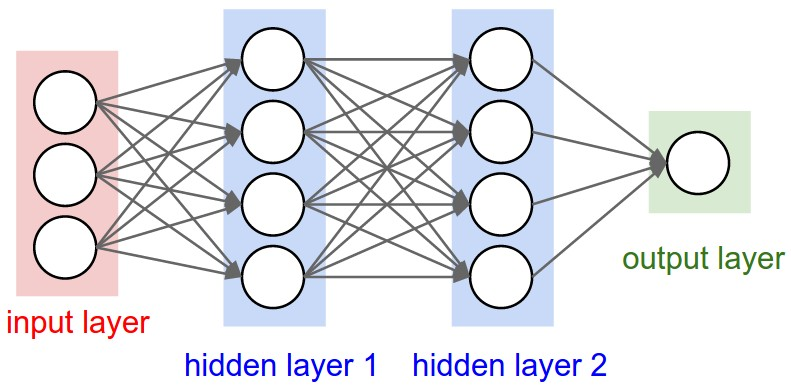
\includegraphics[width=14cm]{NN}\\
  \caption{Basic structure of an neural network, \citet{karpathy2017}}%, 
  \label{fig:nn}
\end{figure}


\subsection{Preprocessing on image}
\label{sec:preprocess}

For the neural network to be able to classify the digits from the images, those images must first be found inside the image. To do this Image processing is required. This is done in 6 steps as seen below:

\begin{enumerate}
\item Find the contour closest to the expected location of the block, calculated in Section \ref{sec:RadonTransform}. This is ilustrated in Figure \ref{fig:sa}. The bubbles have already been filter out of the image in a previous process.
\item Transform the image to become fully rectangle using OpenCv's $four_point_transform$ method. This method applies a four point perspective transform on the image to reshape it into a rectangular form. An example of the final product can be seen in Figure \ref{fig:bp}.
\item Do a horizontal and vertical Radon transform, Section \ref{sec:RadonTransform}, to find and remove the dark box lines on the image, as seen in Figure \ref{fig:ar}.
\item Use the values received from the radon transform to segment the image into the different boxes.
\item Using a custom segmentation algorithm find the pixels most likely to belong to the digit, as seen in Figure \ref{fig:c}.
\item Locate the area the pixels are located in, as seen in Figure \ref{fig:areaLoc}
\item Finally calculate the center of the pixels, recenter and normalize the image area, as seen in Figure \ref{fig:final}
\item Reshape the image into an 28 by 28 greyscalled image to be processed by the neural network.
\end{enumerate}

\begin{figure}
  \centering
  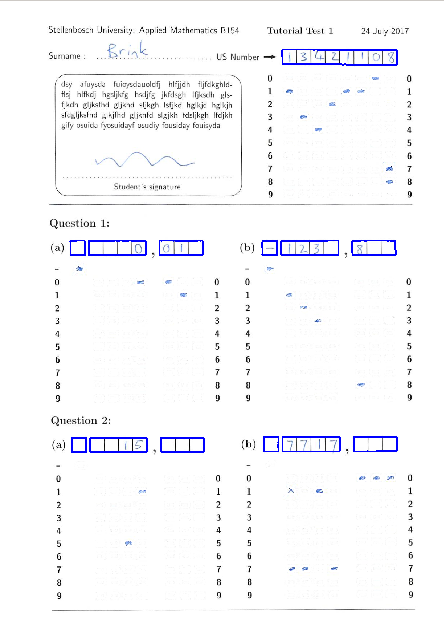
\includegraphics[width=10cm]{DigitScan}\\
  \caption{Image scanned for character areas.}
  \label{fig:sa}
\end{figure}

\begin{figure}
  \centering
  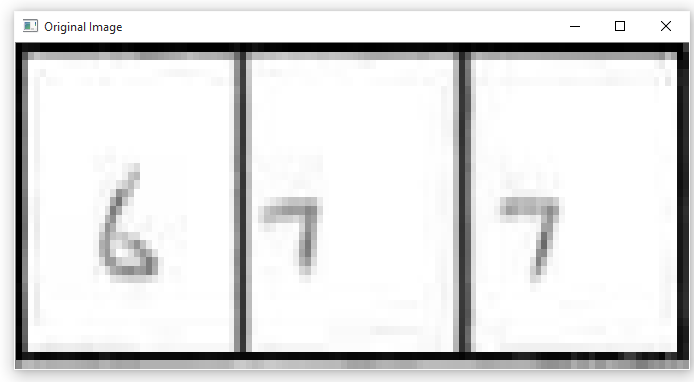
\includegraphics[width=10cm]{BeforeProcessing}\\
  \caption{The found box is then normalized to rectangular shape.}
  \label{fig:bp}
\end{figure}

\begin{figure}
  \centering
  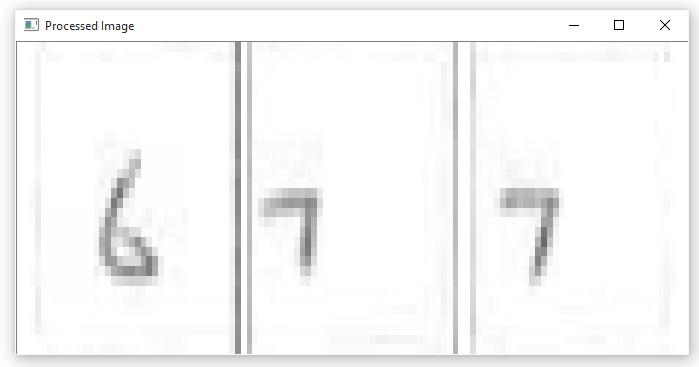
\includegraphics[width=10cm]{AfterRadon}\\
  \caption{a Randon transform then gets applied.}
  \label{fig:ar}
\end{figure}

\begin{figure}
  \centering
  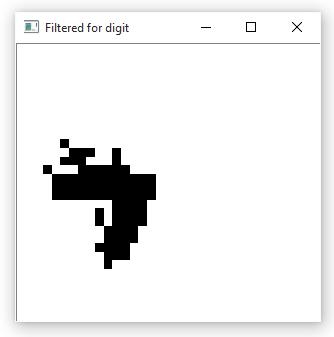
\includegraphics[width=4cm]{Cluster}\\
  \caption{An clustering algorithm is used to find the main cluster in the remaining image.}
  \label{fig:c}
\end{figure}

\begin{figure}
  \centering
  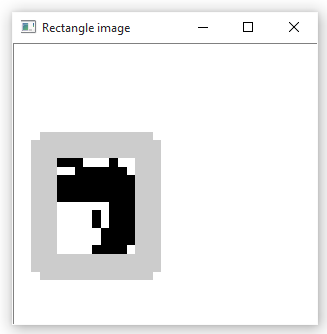
\includegraphics[width=4cm]{DetectArea}\\
  \caption{Area of found cluster.}
  \label{fig:areaLoc}
\end{figure}

\begin{figure}
  \centering
  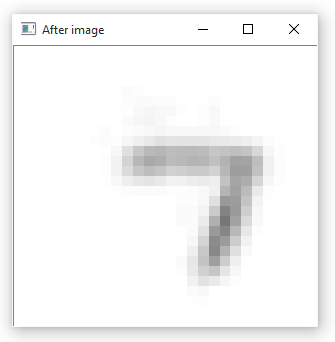
\includegraphics[width=4cm]{TranslateAndScale}\\
  \caption{Final translation and normalization of image.}
  \label{fig:final}
\end{figure}

Each box on the image can now be classified by the neural network and  saved. The new character recognition evidence can now be used in combination with the bubble evidence to make a significantly more accurate estimate of the intended answers of the student. Next all these individual evidence must be combined in a intelligence way to make a accurate prediction. This method will be covered in the next section.

\section{Probabilistic Graphical Models}
\label{sec:PGM}

The last step in this process is to probabilistic determining the true values the student, given all the evidence presented. To do this a probabilistic graphical model(PGM) will be developed.

\subsection{Structure of the graph}

a Probabilistic graphical model(PGM) is a probabilistic model of random variables, where the graph expresses the conditional independence structure between these variables. The type of PGM used in this thesis is a Bayesian network. A Bayesian network models a set of random variables and their conditional dependencies via a directed acyclic graph (DAG). As seen in Figure \ref{fig:pgmDigit}, arrows are used to indicate which variables are conditionally dependent on another. The Figure should be interpreted in the direction which information flows. Firstly a student has a certain digit that he/she wants to portray on the page. This is given by the 'Digit user intended bubble'. There are 10 possible digits to consider and thus the bubble has 10 possible states. This true digit gives rise to the intended bubbles and character that the student wants to write down. The student might sometimes mistakenly think that the first bubble represents 0 and thus even if the intended digit is 0 the intended bubble might be 1. Thus this must also be done in a probabilistic manner. The intended bubbles and character then produces evidence, as seen in Figure \ref{fig:pgmDigit}.  When looking at Figure \ref{fig:column}, it is observed that there are 11 evidence areas to consider. They are the the 10 bubbles and the character block. The process of writing down this digit introduces so noise into the system, due to the fact the student is not always going to write down the digit in exactly the same way. Thus the evidence is also probabilistically linked to the 'intended bubble' or 'intended character' parent distribution. This evidence then gets written down on the paper and is what ultimately influences how the image looks. Each of the bubbles can take one of 4 states as evidence. These states are blank,crossed-out, partially colored in and fully colored in. The character block evidence is an 28 by 28 greyscale image. Thus it can have 28*28*256 possible states, where 256 is the possible pixel intensities of each pixel.

\subsection{Determining the intended digit}
Now that the model constructed the intended digit needs to be estimated, given the image. Thus is done by reasoning from the bottom(image evidence) and upwards to the intended digit. The first step is to process the image that produces the evidence using of image processing. Producing the bubble evidence from the image is described in Chapter \ref{ch:ImageProcessing}. In \ref{sec:preprocess}, the process to extract the character evidence from the image was also described. Using the neural network the probability of intended character can be determined. To determine the intended digit of the student a PGM is constructed.

\begin{figure}
  \centering
  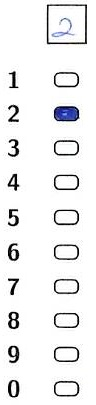
\includegraphics[width=1cm]{column}\\
  \caption{Column representing one digit.}
  \label{fig:column}
\end{figure}

\begin{figure}
  \centering
  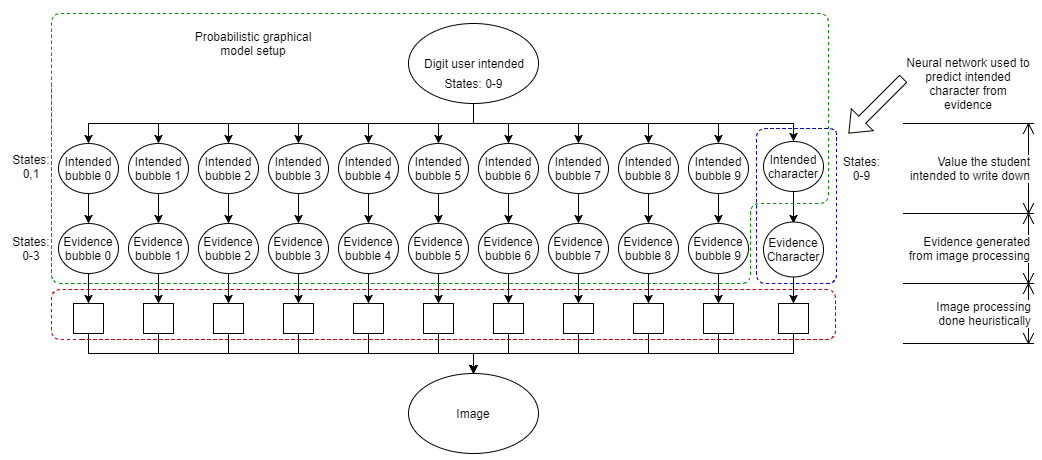
\includegraphics[width=16cm]{pgmDigit}\\
  \caption{Graphical setup of digit generation.}
  \label{fig:pgmDigit}
\end{figure}


\subsection{Training the model}

This subsection still needs to be completed.

As seen in Figure \ref{fig:pgmDigit},the PGM will include the bubble evidence as well as a prior probability that the neural network provides as evidence. Once these values are assigned, the PGM model will infer the intended digit using the probability distribution specified. To do this the conditional probabilities of the PGM, must first be determined from data. This is done by simple.. to be continued.


\subsection{Student number identification}
\label{sec:pgmStudentNum}
To be continued..
\section{Conclusion}

This chapter looked at two machine learning techniques to improve the accuracy with with the system infers the answers written on each scanned test sheet. A method was shown, using a neural network, to estimate the probability of each digit given only the character box as input. Additionally a approach was discussed, using a PGM, to allow the system to make a final prediction of what the student intended to write down given the bubble and character boxes as evidence.

The following chapter will cover the validation and results of the system from weekly grading done for the Applied mathematics department.